\section{Platinen}
Um das Projekt umsetzen zu können, ist es erforderlich einerseits den Mikroprozessor mit den Sensoren zu verbinden und andererseits die Kommunikation zwischen der Speisekarten-App und dem Hexacopter zu können.
Damit diese Funktionen erfüllt werden können, werden zwei Platinen verwendet.

Das wichtigsten Bauteilgruppen der Kommunikationsplatine sind das WLAN-Modul, dieses ermöglicht die Kommunikation zwischen der App und dem Hexacopter und der Spannungsregler. Der Spannungsregler sorgt dafür, dass das WLAN-Modul mit 3.3 V versorgt wird und der Rest der Platine mit 5 V.
Die Hauptplatine beinhaltet ebenso mehrere Bereiche: Den Multiplexer, den Mikroprozessor und die Steckverbindungen für die einzelnen Sensoren.
Der Multiplexer wechslet zwischen der Steuerung der Flugmodi durch die Fernbedienung oder dem Mikroprozessor.
\newpage
\begin{figure}[t]
\begin{centering}
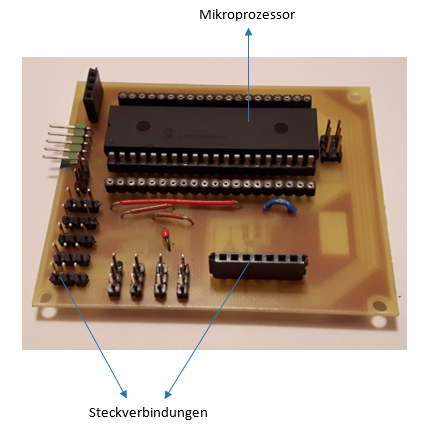
\includegraphics[width = 0.6\textwidth]{Bilder/HP_Top_Beschriftung}
\par\end{centering}
\caption{Sensorplatine Oberseite}
\label{Sensor Platine oben}
\end{figure}

\begin{figure}[b]
\begin{centering}
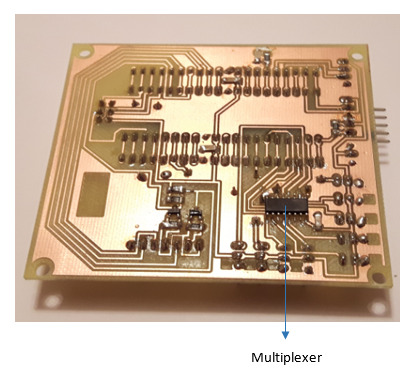
\includegraphics[width = 0.6\textwidth]{Bilder/HP_Bottom_Beschriftung}
\par\end{centering}
\caption{Sensorplatine Unterseite}
\label{Sensor Platine unten}
\end{figure}


\begin{figure}[t]
\begin{centering}
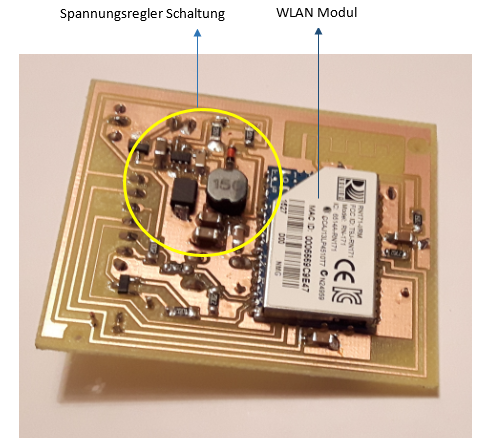
\includegraphics[width = 0.6\textwidth]{Bilder/WP_Bottom_Beschriftung}
\par\end{centering}
\caption{Kommunikationsplatine Unterseite}
\label{WLAN Platine oben}
\end{figure}

\begin{figure}[b]
\begin{centering}
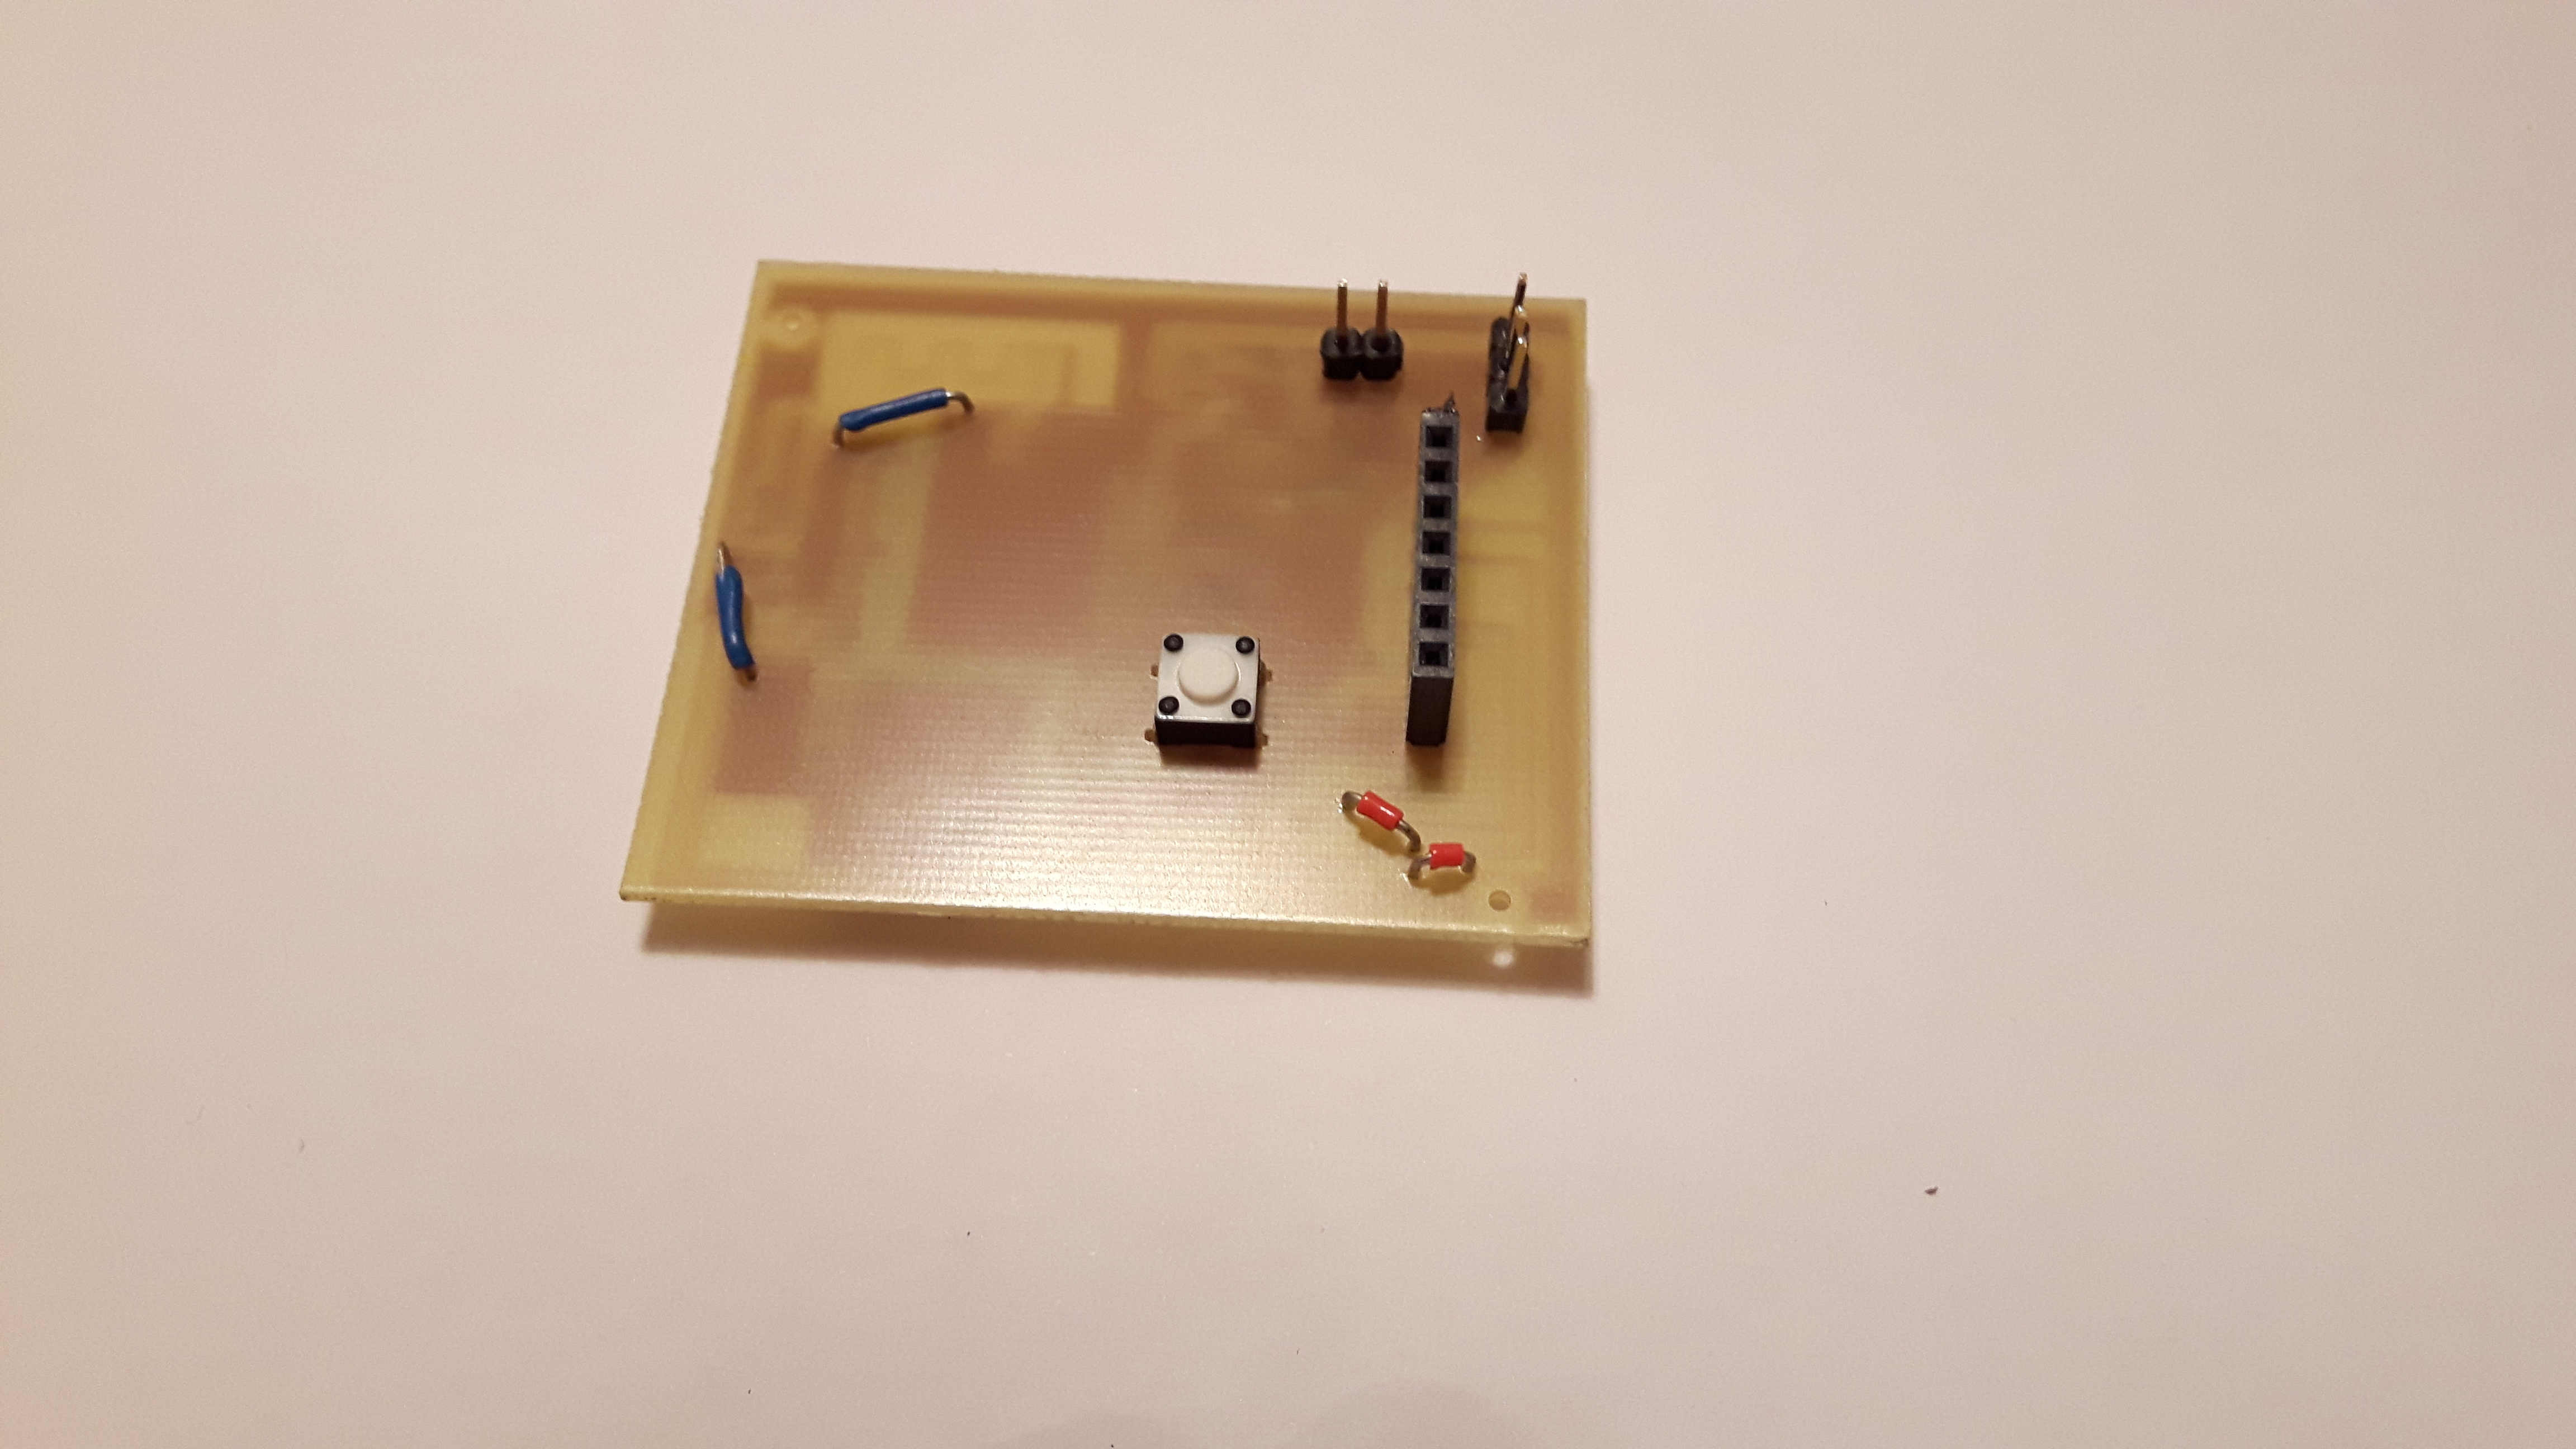
\includegraphics[width = 0.6\textwidth]{Bilder/WP_Top}
\par\end{centering}
\caption{Kommunikationsplatine Oberseite}
\label{WLAN Platine unten}
\end{figure}
